\documentclass[
]{jss}

\usepackage[utf8]{inputenc}

\providecommand{\tightlist}{%
  \setlength{\itemsep}{0pt}\setlength{\parskip}{0pt}}

\author{
Sahir Bhatnagar *\\McGill University \And Maxime Turgeon *\\University of Manitoba \AND Jesse Islam\\McGill University \And James Hanley\\McGill University \And Olli Saarela\\University of Toronto
}
\title{\pkg{casebase}: An Alternative Framework For Survival Analysis}

\Plainauthor{Sahir Bhatnagar *, Maxime Turgeon *, Jesse Islam, James Hanley, Olli Saarela}
\Plaintitle{casebase: An Alternative Framework For Survival Analysis}
\Shorttitle{\pkg{casebase}: An Alternative Framework For Survival Analysis}

\Abstract{
The abstract of the article. * joint co-authors
}

\Keywords{keywords, not capitalized, \proglang{Java}}
\Plainkeywords{keywords, not capitalized, Java}

%% publication information
%% \Volume{50}
%% \Issue{9}
%% \Month{June}
%% \Year{2012}
%% \Submitdate{}
%% \Acceptdate{2012-06-04}

\Address{
    Sahir Bhatnagar *\\
  McGill University\\
  1020 Pine Avenue West Montreal, QC, Canada H3A 1A2\\
  E-mail: \email{sahir.bhatnagar@mail.mcgill.ca}\\
  URL: \url{http://sahirbhatnagar.com/}\\~\\
      Maxime Turgeon *\\
  University of Manitoba\\
  186 Dysart Road Winnipeg, MB, Canada R3T 2N2\\
  E-mail: \email{max.turgeon@umanitoba.ca}\\
  URL: \url{http://maxturgeon.ca/}\\~\\
      Jesse Islam\\
  McGill University\\
  1020 Pine Avenue West Montreal, QC, Canada H3A 1A2\\
  E-mail: \email{jesse.islam@mail.mcgill.ca}\\
  
      James Hanley\\
  McGill University\\
  1020 Pine Avenue West Montreal, QC, Canada H3A 1A2\\
  E-mail: \email{james.hanley@mcgill.ca}\\
  URL: \url{http://www.medicine.mcgill.ca/epidemiology/hanley/}\\~\\
      Olli Saarela\\
  University of Toronto\\
  Dalla Lana School of Public Health, 155 College Street, 6th floor,
  Toronto, Ontario M5T 3M7, Canada\\
  E-mail: \email{olli.saarela@utoronto.ca}\\
  URL: \url{http://individual.utoronto.ca/osaarela/}\\~\\
  }

% Pandoc header

\usepackage{amsmath} \usepackage{longtable}

\begin{document}

\hypertarget{introduction}{%
\section{Introduction}\label{introduction}}

The purpose of the \pkg{casebase} package is to provide practitioners
with an easy-to-use software tool to predict the risk (or cumulative
incidence (CI)) of an event, for a particular patient. The following
points should be noted:

\begin{enumerate}
\def\labelenumi{\arabic{enumi}.}
\tightlist
\item
  Time matching/risk set sampling (including Cox partial likelihood)
  eliminates the baseline hazard from the likelihood expression for the
  hazard ratios
\item
  If, however, the absolute risks are of interest, they have to be
  recovered using the semi-parametric Breslow estimator
\item
  Alternative approaches for fitting flexible hazard models for
  estimating absolute risks, not requiring this two-step approach? Yes!
  \citep{hanley2009fitting}
\end{enumerate}

\citep{hanley2009fitting} propose a fully parametric hazard model that
can be fit via logistic regression. From the fitted hazard function,
cumulative incidence and, thus, risk functions of time, treatment and
profile can be easily derived.

\begin{table}
  \begin{tabular}{p{1.8in}lll}
\hline
    &  Parameters &  Density \proglang{R} function & \code{dist}\\
    & {\footnotesize{(location in \code{\color{red}{red}})}} & & \\
\hline
    Exponential & \code{\color{red}{rate}}             & \code{dexp}   & \code{"exp"} \\
    Weibull (accelerated failure time)     & \code{shape, {\color{red}{scale}}}     & \code{dweibull} & \code{"weibull"} \\
    Weibull (proportional hazards)     & \code{shape, {\color{red}{scale}}}     & \code{dweibullPH} & \code{"weibullPH"} \\
    Gamma       & \code{shape, \color{red}{rate}}      & \code{dgamma} & \code{"gamma"}\\
    Log-normal  & \code{{\color{red}{meanlog}}, sdlog}   & \code{dlnorm} & \code{"lnorm"}\\
    Gompertz    & \code{shape, {\color{red}{rate}}}      & \code{dgompertz} & \code{"gompertz"} \\
    Log-logistic & \code{shape, {\color{red}{scale}}}   & \code{dllogis} & \code{"llogis"}\\
    Generalized gamma (Prentice 1975)   & \code{{\color{red}{mu}}, sigma, Q} & \code{dgengamma} & \code{"gengamma"} \\
    Generalized gamma (Stacy 1962)& \code{shape, {\color{red}{scale}}, k} & \code{dgengamma.orig} & \code{"gengamma.orig"} \\
    Generalized F     (stable)    & \code{{\color{red}{mu}}, sigma, Q, P} & \code{dgenf} & \code{"genf"} \\
    Generalized F     (original)  & \code{{\color{red}{mu}}, sigma, s1, s2} & \code{dgenf.orig} & \code{"genf.orig"} \\
\hline
  \end{tabular}
  \caption{Built-in parametric survival distributions in \pkg{flexsurv}.}
  \label{tab:dists}
\end{table}

\hypertarget{theoretical-details}{%
\section{Theoretical details}\label{theoretical-details}}

As discussed in Hanley \& Miettinen \citeyearpar{hanley2009fitting}, the
key idea behind case-base sampling is to discretize the study base into
an infinite amount of \emph{person moments}. These person moments are
indexed by both an individual in the study and a time point, and
therefore each person moment has a covariate profile, an exposure status
and an outcome status attached to it. We note that there is only a
finite number of person moments associated with the event of interest
(what Hanley \& Miettinen call the \emph{case series}). The case-base
sampling refers to the sampling from the base of a representative finite
sample called the \emph{base series}.

As shown by Saarela \& Arjas \citeyearpar{saarela2015non} (and further
expanded in Saarela \citeyearpar{saarela2016case}), writing the
likelihood arising from this data-generating mechanism using the
framework of non-homogeneous Poisson processes, we eventually reach an
expression where each person-moment's contribution is of the form
\[\frac{h(t)^{dN(t)}}{\rho(t) + h(t)},\] where \(N(t)\) is the counting
process associated with the event of interest, \(h(t)\) is the
corresponding hazard function, and \(\rho(t)\) is the hazard function
for the Poisson process associated with case-base sampling. This
parametric form suggests that we can readily estimate log-hazards of the
form \(\log(h(t)) = g(t; X)\) using logistic regression, where each
observation corresponds to a person moment, the function \(g(t; X)\) is
linear in a finite number of parameters, and where we treat
\(-\log(\rho(t))\) as an offset.

In Hanley \& Miettinen \citeyearpar{hanley2009fitting}, the authors
suggest performing case-base sampling \emph{uniformly}, i.e.~to sample
the base series uniformly from the study base. In terms of Poisson
processes, this sampling strategy corresponds essentially to a
time-homogeneous Poisson process with intensity equal to \(b/B\), where
\(b\) is the number of sampled observations in the base series, and
\(B\) is the total population-time for the study base. More complex
examples are also available; see for example Saarela \& Arjas
\citeyearpar{saarela2015non}, where the probabilities of the sampling
mechanism are proportional to the cardiovascular disease event rate
given by the Framingham score.

The \texttt{casebase} package fits the family of hazard functions of the
form

\[ h(t;X) = \exp[g(t;X)] \] where \(t\) denotes time and \(X\), the
individual's covariate profile. Different functions of \(t\) lead to
different parametric hazard models. The simplest of these models is the
one-parameter exponential distribution which is obtained by taking the
hazard function to be constant over the range of \(t\).

\[ h(t;X) = \exp(\beta_0 + \beta_1 X) \]

The instantaneous failure rate is independent of \(t\), so that the
conditional chance of failure in a time interval of specified length is
the same regardless of how long the individual has been in the study.
This is also known as the \emph{memoryless property} (Kalbfleisch and
Prentice, 2002).

The Gompertz hazard model is given by including a linear term for time:

\[ h(t;X)  = \exp(\beta_0 + \beta_1 t + \beta_2 X) \]

Use of \(\log(t)\) yields the Weibull hazard which allows for a power
dependence of the hazard on time (Kalbfleisch and Prentice, 2002):

\[ h(t;X)  = \exp(\beta_0 + \beta_1 \log(t) + \beta_2 X) \]

For competing-risk analyses with \(J\) possible events, we can show that
each person-moment's contribution of the likelihood is of the form

\[\frac{h_j(t)^{dN_j(t)}}{\rho(t) + \sum_{j=1}^Jh_j(t)},\]

where \(N_j(t)\) is the counting process associated with the event of
type \(j\) and \(h_j(t)\) is the corresponding hazard function. As may
be expected, this functional form is similar to the terms appearing in
the likelihood function for multinomial
regression.\footnote{Specifically, it corresponds to the following parametrization: \begin{align*} \log\left(\frac{P(Y=j \mid X)}{P(Y = J \mid X)}\right) = X^T\beta_j, \qquad j = 1,\ldots, J-1\end{align*}}

\hypertarget{implementation-details}{%
\section{Implementation details}\label{implementation-details}}

The functions in the casebase package can be divided into two
categories: 1) data visualization, in the form of population-time plots;
and 2) parametric modeling. We explicitly aimed at being compatible with
both \code{data.frame}s and \code{data.table}s. This is evident in some
of the coding choices we made, and it is also reflected in our unit
tests.

\hypertarget{population-time-plots}{%
\subsection{Population-time plots}\label{population-time-plots}}

\hypertarget{parametric-modeling}{%
\subsection{Parametric modeling}\label{parametric-modeling}}

The parametric modeling step was separated into three parts:

\begin{enumerate}
\def\labelenumi{\arabic{enumi}.}
\tightlist
\item
  case-base sampling;
\item
  estimation of the smooth hazard function;
\item
  calculation of the risk function.
\end{enumerate}

By separating the sampling and estimation functions, we allowed the
possibility of users implementing more complex sampling scheme, as
described in Saarela \citeyearpar{saarela2016case}.

The sampling scheme selected for \code{sampleCaseBase} was described in
Hanley and Miettinen \citeyearpar{hanley2009fitting}: we first sample
along the ``person'' axis, proportional to each individual's total
follow-up time, and then we sample a moment uniformly over their
follow-up time. This sampling scheme is equivalent to the following
picture: imagine representing the total follow-up time of all
individuals in the study along a single dimension, where the follow-up
time of the next individual would start exactly when the follow-up time
of the previous individual ends. Then the base series could be sampled
uniformly from this one-dimensional representation of the overall
follow-up time. In any case, the output is a dataset of the same class
as the input, where each row corresponds to a person-moment. The
covariate profile for each such person-moment is retained, and an offset
term is added to the dataset. This output could then be used to fit a
smooth hazard function, or for visualization of the base series.

The fitting function \code{fitSmoothHazard} starts by looking at the
class of the dataset: if it was generated from \code{sampleCaseBase}, it
automatically inherited the class \code{cbData}. If the dataset supplied
to \code{fitSmoothHazard} does not inherit from \code{cbData}, then the
fitting function starts by calling \code{sampleCaseBase} to generate the
base series. In other words, the occasional user can bypass
\code{sampleCaseBase} altogether and only worry about the fitting
function \code{fitSmoothHazard}.

The fitting function retains the familiar formula interface of
\code{glm}. The left-hand side of the formula should be the name of the
column corresponding to the event type. The right-hand side can be any
combination of the covariates, along with an explicit functional form
for the time variable. Note that non-proportional hazard models can be
achieved at this stage by adding an interaction term involving time. The
offset term does not need to be specified by the user, as it is
automatically added to the formula.

To fit the hazard function, we provide several approaches that are
available via the \code{family} parameter. These approaches are:

\begin{itemize}
\tightlist
\item
  \code{glm}: This is the familiar logistic regression.
\item
  \code{glmnet}: This option allows for variable selection using Lasso
  or elastic-net. This functionality is provided through the
  \code{glmnet} package \citep{friedman2010jss}.
\item
  \code{gam}: This option provides support for \emph{Generalized
  Additive Models} via the \code{gam} package
  \citep{hastie1987generalized}.
\item
  \code{gbm}: This option provides support for \emph{Gradient Boosted
  Trees} via the \code{gbm} package. This feature is still experimental.
\end{itemize}

In the case of multiple events, the hazard is fitted via multinomial
regression as performed by the \pkg{VGAM} package. This package was
selected for its ability to fit multinomial regression models with an
offset.

Once a model-fit object has been returned by \code{fitSmoothHazard}, all
the familiar summary and diagnostic functions are available:
\code{print}, \code{summary}, \code{predict}, \code{plot}, etc. Our
package provides one more functionality: it computes risk functions from
the model fit. For the case of a single event, it uses the familiar
identity \[S(t) = \exp\left(-\int_0^t h(u;X) du\right).\] The integral
is computed using either the \code{stats::integrate} function or
Monte-Carlo integration. The risk function (or cumulative incidence
function) is then defined as

\[ CI(t) = 1 - S(t).\]

For the case of a competing-event analysis, the event-specific risk is
computed using the following procedure: first, we compute the overall
survival function (i.e.~for all event types):

\[ S(t) = \exp\left(-\int_0^t H(u;X) du\right),\qquad H(t;X) = \sum_{j=1}^J h_j(t;X).\]
From this, we can derive the event-specific subdensities:

\[ f_j(t) = h_j(t)S(t).\]

Finally, by integrating these subdensities, we obtain the event-specific
cumulative incidence functions:

\[ CI_j(t) = \int_0^t f_j(u)du.\]

We created \code{absoluteRisk} as an \code{S3} generic, with methods for
the different types of outputs of \code{fitSmoothHazard}. The method
dispatch system of \proglang{R} then takes care of matching the correct
output to the correct methodology for calculating the cumulative
incidence function, without the user's intervention.

In the following sections, we illustrate these functionalities in the
context of three case studies.

\hypertarget{case-study-1european-randomized-study-of-prostate-cancer-screening}{%
\section{Case study 1--European Randomized Study of Prostate Cancer
Screening}\label{case-study-1european-randomized-study-of-prostate-cancer-screening}}

To introduce the different features available, we make use of the
European Randomized Study of Prostate Cancer Screening data; this
dataset is available through the \pkg{casebase} package:

\begin{CodeChunk}

\begin{CodeInput}
R> data(ERSPC)
R> ERSPC$ScrArm <- factor(ERSPC$ScrArm, 
R>                        levels = c(0,1), 
R>                        labels = c("Control group", "Screening group"))
\end{CodeInput}
\end{CodeChunk}

The results of this study were published by {[}schroder2009screening{]}.
This data was obtained using the approach described in
{[}liu2014recovering{]}.

Population time plots can be extremely informative graphical displays of
survival data. They should be the first step in an exploratory data
analysis. We facilitate this task in the \pkg{casebase} package using
the \code{popTime} function. We first create the necessary dataset for
producing the population time plots, and we can produce the plot by
using the corresponding \code{plot} method:

\begin{CodeChunk}

\begin{CodeInput}
R> pt_object <- casebase::popTime(ERSPC, event = "DeadOfPrCa")
R> plot(pt_object)
\end{CodeInput}
\end{CodeChunk}

We can also create exposure stratified plots by specifying the
\code{exposure} argument in the \code{popTime} function:

\begin{CodeChunk}

\begin{CodeInput}
R> pt_object_strat <- casebase::popTime(ERSPC, 
R>                                      event = "DeadOfPrCa", 
R>                                      exposure = "ScrArm")
R> plot(pt_object_strat)
\end{CodeInput}
\end{CodeChunk}

We can also plot them side-by-side using the \code{ncol} argument:

\begin{CodeChunk}

\begin{CodeInput}
R> plot(pt_object_strat, ncol = 2)
\end{CodeInput}
\end{CodeChunk}

First, we fit a Cox model to the data, examine the hazard ratio for the
screening group (relative to the control group), and plot the cumulative
incidence function (CIF).

\begin{CodeChunk}

\begin{CodeInput}
R> cox_model <- survival::coxph(Surv(Follow.Up.Time, DeadOfPrCa) ~ ScrArm, 
R>                              data = ERSPC)
R> summary(cox_model)
\end{CodeInput}
\end{CodeChunk}

We can plot the CIF for each group:

\begin{CodeChunk}

\begin{CodeInput}
R> new_data <- data.frame(ScrArm = c("Control group", "Screening group"),
R>                        ignore = 99)
R> 
R> plot(survfit(cox_model, newdata = new_data),
R>      xlab = "Years since Randomization", 
R>      ylab = "Cumulative Incidence", 
R>      fun = "event",
R>      xlim = c(0,15), conf.int = FALSE, col = c("red","blue"), 
R>      main = sprintf("Estimated Cumulative Incidence (risk) of Death from Prostate 
R>                     Cancer Screening group Hazard Ratio: %.2g (%.2g, %.2g)",
R>                     exp(coef(cox_model)), 
R>                     exp(confint(cox_model))[1], 
R>                     exp(confint(cox_model))[2]))
R> legend("topleft", 
R>        legend = c("Control group", "Screening group"), 
R>        col = c("red","blue"),
R>        lty = c(1, 1), 
R>        bg = "gray90")
\end{CodeInput}
\end{CodeChunk}

Next we fit several models using case-base sampling. The models we fit
differ in how we choose to model time.

The \code{fitSmoothHazard} function provides an estimate of the hazard
function \(h(x, t)\) is the hazard function, where \(t\) denotes the
numerical value of a point in prognostic/prospective time and \(x\) is
the realization of the vector \(X\) of variates based on the patient's
profile and intervention (if any).

\begin{CodeChunk}

\begin{CodeInput}
R> casebase_exponential <- casebase::fitSmoothHazard(DeadOfPrCa ~ ScrArm, 
R>                                                   data = ERSPC, 
R>                                                   ratio = 100)
R> 
R> summary(casebase_exponential)
R> exp(coef(casebase_exponential)[2])
R> exp(confint(casebase_exponential)[2,])
\end{CodeInput}
\end{CodeChunk}

The \code{absoluteRisk} function provides an estimate of the cumulative
incidence curves for a specific risk profile using the following
equation:

\[ CI(x, t) = 1 - \exp\left( - \int_0^t h(x, u) \textrm{d}u \right) \]

In the plot below, we overlay the estimated CIF from the casebase
exponential model on the Cox model CIF:

\begin{CodeChunk}

\begin{CodeInput}
R> smooth_risk_exp <- casebase::absoluteRisk(object = casebase_exponential, 
R>                                           time = seq(0,15,0.1), 
R>                                           newdata = new_data)
R> 
R> plot(survfit(cox_model, newdata = new_data),
R>      xlab = "Years since Randomization", 
R>      ylab = "Cumulative Incidence", 
R>      fun = "event",
R>      xlim = c(0,15), conf.int = FALSE, col = c("red","blue"), 
R>      main = sprintf("Estimated Cumulative Incidence (risk) of Death from Prostate 
R>                     Cancer Screening group Hazard Ratio: %.2g (%.2g, %.2g)",
R>                     exp(coef(cox_model)), 
R>                     exp(confint(cox_model))[1], 
R>                     exp(confint(cox_model))[2]))
R> lines(smooth_risk_exp[,1], smooth_risk_exp[,2], col = "red", lty = 2)
R> lines(smooth_risk_exp[,1], smooth_risk_exp[,3], col = "blue", lty = 2)
R> 
R> 
R> legend("topleft", 
R>        legend = c("Control group (Cox)","Control group (Casebase)",
R>                   "Screening group (Cox)", "Screening group (Casebase)"), 
R>        col = c("red","red", "blue","blue"),
R>        lty = c(1, 2, 1, 2), 
R>        bg = "gray90")
\end{CodeInput}
\end{CodeChunk}

As we can see, the exponential model is not a good fit. Based on what we
observed in the population time plot, where more events are observed
later on in time, this poor fit is expected. A constant hazard model
would overestimate the cumulative incidence earlier on in time, and
underestimate it later on; this is what we see on the cumulative
incidence plot. This example demonstrates the benefits of population
time plots as an exploratory analysis tool.

Next we enter time linearly into the model:

\begin{CodeChunk}

\begin{CodeInput}
R> casebase_time <- fitSmoothHazard(DeadOfPrCa ~ Follow.Up.Time + ScrArm, 
R>                                  data = ERSPC, 
R>                                  ratio = 100)
R> 
R> summary(casebase_time)
R> exp(coef(casebase_time))
R> exp(confint(casebase_time))
\end{CodeInput}
\end{CodeChunk}

\begin{CodeChunk}

\begin{CodeInput}
R> smooth_risk_time <- casebase::absoluteRisk(object = casebase_time, 
R>                                           time = seq(0,15,0.1), 
R>                                           newdata = new_data)
R> 
R> plot(survfit(cox_model, newdata = new_data),
R>      xlab = "Years since Randomization", 
R>      ylab = "Cumulative Incidence", 
R>      fun = "event",
R>      xlim = c(0,15), conf.int = FALSE, col = c("red","blue"), 
R>      main = sprintf("Estimated Cumulative Incidence (risk) of Death from Prostate 
R>                     Cancer Screening group Hazard Ratio: %.2g (%.2g, %.2g)",
R>                     exp(coef(cox_model)), 
R>                     exp(confint(cox_model))[1], 
R>                     exp(confint(cox_model))[2]))
R> lines(smooth_risk_time[,1], smooth_risk_time[,2], col = "red", lty = 2)
R> lines(smooth_risk_time[,1], smooth_risk_time[,3], col = "blue", lty = 2)
R> 
R> legend("topleft", 
R>        legend = c("Control group (Cox)","Control group (Casebase)",
R>                   "Screening group (Cox)", "Screening group (Casebase)"), 
R>        col = c("red","red", "blue","blue"),
R>        lty = c(1, 2, 1, 2), 
R>        bg = "gray90")
\end{CodeInput}
\end{CodeChunk}

We see that the Weibull model leads to a better fit.

Next we try to enter a smooth function of time into the model using the
\code{splines} package:

\begin{CodeChunk}

\begin{CodeInput}
R> casebase_splines <- fitSmoothHazard(DeadOfPrCa ~ bs(Follow.Up.Time) + ScrArm, 
R>                                     data = ERSPC, 
R>                                     ratio = 100)
R> 
R> summary(casebase_splines)
R> exp(coef(casebase_splines))
R> exp(confint(casebase_splines))
\end{CodeInput}
\end{CodeChunk}

\begin{CodeChunk}

\begin{CodeInput}
R> smooth_risk_splines <- absoluteRisk(object = casebase_splines, 
R>                                     time = seq(0,15,0.1), 
R>                                     newdata = new_data)
R> 
R> plot(survfit(cox_model, newdata = new_data),
R>      xlab = "Years since Randomization", 
R>      ylab = "Cumulative Incidence", 
R>      fun = "event",
R>      xlim = c(0,15), conf.int = FALSE, col = c("red","blue"), 
R>      main = sprintf("Estimated Cumulative Incidence (risk) of Death from Prostate 
R>                     Cancer Screening group Hazard Ratio: %.2g (%.2g, %.2g)",
R>                     exp(coef(cox_model)), 
R>                     exp(confint(cox_model))[1], 
R>                     exp(confint(cox_model))[2]))
R> lines(smooth_risk_splines[,1], smooth_risk_splines[,2], col = "red", lty = 2)
R> lines(smooth_risk_splines[,1], smooth_risk_splines[,3], col = "blue", lty = 2)
R> 
R> legend("topleft", 
R>        legend = c("Control group (Cox)","Control group (Casebase)",
R>                   "Screening group (Cox)", "Screening group (Casebase)"), 
R>        col = c("red","red", "blue","blue"),
R>        lty = c(1, 2, 1, 2), 
R>        bg = "gray90")
\end{CodeInput}
\end{CodeChunk}

It looks like the best fit.

Since we are within the GLM framework, we can easily test for which
model better fits the data using a Likelihood Ratio Test (LRT). The null
hypothesis here is that the linear model is just as good as the larger
(in terms of number of parameters) splines model.

\begin{CodeChunk}

\begin{CodeInput}
R> anova(casebase_time, casebase_splines, test = "LRT")
\end{CodeInput}
\end{CodeChunk}

As expected, we see that splines model provides a better fit.

\hypertarget{case-study-2bone-marrow-transplant}{%
\section{Case study 2--Bone-marrow
transplant}\label{case-study-2bone-marrow-transplant}}

The next example shows how case-base sampling can also be used in the
context of a competing risk analysis. For illustrative purposes, we will
use the same data that was used in Scrucca \emph{et al}
\citeyearpar{scrucca2010regression}. The data was downloaded from the
main author's website, and it is also available as part of the
\pkg{casebase} package.

\begin{CodeChunk}

\begin{CodeInput}
R> data(bmtcrr)
\end{CodeInput}
\end{CodeChunk}

The data contains information on 177 patients who received a stem-cell
transplant for acute leukemia. The event of interest is relapse, but
other competing causes (e.g.~transplant-related death) were also
recorded Several covariates were also captured at baseline: sex, disease
type (acute lymphoblastic or myeloblastic leukemia, abbreviated as ALL
and AML, respectively), disease phase at transplant (Relapse, CR1, CR2,
CR3), source of stem cells (bone marrow and peripheral blood, coded as
BM+PB, or only peripheral blood, coded as PB), and age. A summary of
these baseline characteristics appear in Table \ref{tab:table1bmtcrr}.
We note that the statistical summaries were generated differently for
different variable types: for continuous variables, we gave the range,
followed by the mean and standard deviation; for categorical variables,
we gave the counts for each category.

\begin{table}[ht]
\centering
\begin{tabular}{lll}
  \hline
Variable & Description & Statistical summary \\ 
  \hline
Sex & Sex & M=Male (100) \\ 
   &  & F=Female (77) \\ 
  D & Disease & ALL (73) \\ 
   &  & AML (104) \\ 
  Phase & Phase & CR1 (47) \\ 
   &  & CR2 (45) \\ 
   &  & CR3 (12) \\ 
   &  & Relapse (73) \\ 
  Source & Type of transplant & BM+PB (21) \\ 
   &  & PB (156) \\ 
  Age & Age of patient (years) & 4–62 \\ 
   &  & 30.47 (13.04) \\ 
  Ftime & Failure time (months) & 0.13–131.77 \\ 
   &  & 20.28 (30.78) \\ 
  Status & Status indicator & 0=censored (46) \\ 
   &  & 1=relapse (56) \\ 
   &  & 2=competing event (75) \\ 
   \hline
\end{tabular}
\caption{Baseline characteristics of patients in the stem-cell transplant study.}
\label{tab:table1bmtcrr}
\end{table}

In order to try and visualize the incidence density of relapse, we can
look at the corresponding population-time plot. In Figure
\ref{fig:compPop1}, failure times associated with relapse are
highlighted on the plot using red points, while Figure
\ref{fig:compPop2} provides a similar population-time plot for competing
events.

Our main objective is to compute the absolute risk of relapse for a
given set of covariates. First, we fit a smooth hazard to the data; for
the sake of this example, we opted for a linear term for time:

\begin{CodeChunk}

\begin{CodeInput}
R> model_cb <- fitSmoothHazard(
R>     Status ~ ftime + Sex + D + Phase + Source + Age, 
R>     data = bmtcrr, 
R>     ratio = 100, 
R>     time = "ftime")
\end{CodeInput}
\end{CodeChunk}

From the fit object, we can extract both the hazard ratios and their
corresponding confidence intervals:

As we can see, the only significant hazard ratio is the one associated
with the phase of the disease at transplant. More precisely, being in
relapse at transplant is associated with a hazard ratio of 3.92 when
compared to CR1.

Given our estimate of the hazard function, we can compute the absolute
risk curve for a fixed covariate profile. We performed this computation
for a 35 year old woman who received a stem-cell transplant from
peripheral blood at relapse. We compared the absolute risk curve for
such a woman with acute lymphoblastic leukemia with that for a similar
woman with acute myeloblastic leukemia. Figure \ref{fig:compAbsrisk}
shows these two curves as a function of time. This figure also shows the
Kaplan-Meier estimate fitted to the two disease groups (ignoring the
other covariates).

\begin{CodeChunk}

\begin{CodeInput}
R> # Pick 100 equidistant points between 0 and 60 months
R> time_points <- seq(0, 60, length.out = 50)
R> 
R> # Data.frame containing risk profile
R> newdata <- data.frame("Sex" = factor(c("F", "F"), 
R>                                      levels = levels(bmtcrr[,"Sex"])),
R>                       "D" = c("ALL", "AML"),
R>                       "Phase" = factor(c("Relapse", "Relapse"), 
R>                                        levels = levels(bmtcrr[,"Phase"])),
R>                       "Age" = c(35, 35),
R>                       "Source" = factor(c("PB", "PB"), 
R>                                         levels = levels(bmtcrr[,"Source"])))
R> 
R> # Estimate absolute risk curve
R> risk_cb <- absoluteRisk(object = model_cb, time = time_points,
R>                         method = "numerical", newdata = newdata)
\end{CodeInput}
\end{CodeChunk}

\hypertarget{case-study-3the-cancer-genome-atlas}{%
\section{Case study 3--The Cancer Genome
Atlas}\label{case-study-3the-cancer-genome-atlas}}

\begin{itemize}
\tightlist
\item
  Glmnet and TCGA data
\end{itemize}

\hypertarget{case-study-4stanford-heart-transplant-data}{%
\section{Case study 4--Stanford Heart Transplant
Data}\label{case-study-4stanford-heart-transplant-data}}

Although the previous case studies provide a broad overview of the
capabilities of \pkg{casebase}, they all have two properties in common:

\begin{itemize}
  \item All covariates are fixed, i.e. they do not change over time;
  \item The estimated hazard functions satisfy the "proportional hazard" assumption.
\end{itemize}

The purpose of the next case study is to show how \pkg{casebase} can
also be used for survival analysis problems that do not share these
properties. To this end, we will use the Stanford Heart Transplant Data
\citep[\citet{crowley1977covariance}]{clark1971cardiac}; we will use the
version available in the \pkg{survival} package.

\begin{CodeChunk}

\begin{CodeInput}
R> library(survival)
R> library(casebase)
R> 
R> stanford_popTime <- popTime(jasa, time = "futime", 
R+                             event = "fustat")
R> plot(stanford_popTime)
\end{CodeInput}


\begin{center}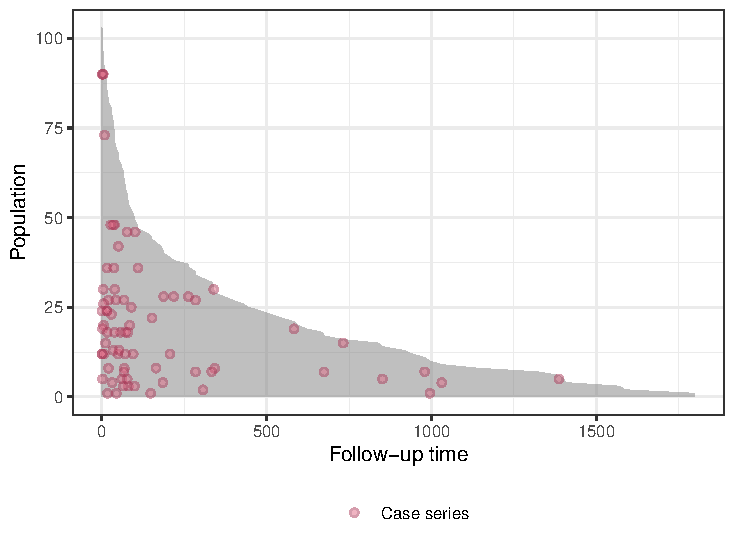
\includegraphics{../figures/stanford-poptime-1} \end{center}

\end{CodeChunk}

Since the exposure is time dependent, we need to manually define the
exposure variable \emph{after} case-base sampling and \emph{before}
fitting the hazard function. For this reason, we will use the
\texttt{sampleCaseBase} function directly.

\begin{CodeChunk}

\begin{CodeInput}
R> library(tidyverse)
R> library(lubridate)
R> 
R> cb_data <- sampleCaseBase(jasa, time = "futime", 
R+                           event = "fustat", ratio = 10)
\end{CodeInput}
\end{CodeChunk}

Next, we will compute the number of days from acceptance into the
program to transplant, and we use this variable to determine whether
each population-moment is exposed or not.

\begin{CodeChunk}

\begin{CodeInput}
R> # Define exposure variable
R> cb_data <- mutate(cb_data,
R+                   txtime = time_length(accept.dt %--% tx.date, 
R+                                        unit = "days"),
R+                   exposure = case_when(
R+                     is.na(txtime) ~ 0L,
R+                     txtime > futime ~ 0L,
R+                     txtime <= futime ~ 1L
R+                   ))
\end{CodeInput}
\end{CodeChunk}

Finally, we can fit the hazard using various linear predictors.

\begin{CodeChunk}

\begin{CodeInput}
R> library(splines)
R> # Fit several models
R> fit1 <- fitSmoothHazard(fustat ~ exposure,
R+                         data = cb_data, time = "futime")
R> fit2 <- fitSmoothHazard(fustat ~ exposure + futime,
R+                         data = cb_data, time = "futime")
R> fit3 <- fitSmoothHazard(fustat ~ exposure + bs(futime),
R+                         data = cb_data, time = "futime")
R> fit4 <- fitSmoothHazard(fustat ~ exposure*bs(futime),
R+                         data = cb_data, time = "futime")
\end{CodeInput}
\end{CodeChunk}

Note that the fourth model (i.e. \texttt{fit4}) includes an interaction
term between exposure and follow-up time. In other words, this model no
longer exhibit proportional hazards. We can then compare the goodness of
fit of these four models using the Akaike Information Criterion (AIC).

\begin{CodeChunk}

\begin{CodeInput}
R> # Compute AIC
R> c("Model1" = AIC(fit1),
R+   "Model2" = AIC(fit2),
R+   "Model3" = AIC(fit3),
R+   "Model4" = AIC(fit4))
\end{CodeInput}

\begin{CodeOutput}
#> Model1 Model2 Model3 Model4 
#>    796    760    730    728
\end{CodeOutput}
\end{CodeChunk}

As we can, the best fit is the fourth model. By visualizing the hazard
functions for both exposed and unexposed individuals, we can more
clearly see how the hazards are no longer proportional.

\begin{CodeChunk}

\begin{CodeInput}
R> # Compute hazards---
R> # First, create a list of time points for both exposure status
R> hazard_data <- expand.grid(exposure = c(0, 1),
R+                            futime = seq(0, 1000,
R+                                         length.out = 100))
R> # Set the offset to zero
R> hazard_data$offset <- 0 
R> # Use predict to get the fitted values, and exponentiate to 
R> # transform to the right scale
R> hazard_data$hazard = exp(predict(fit4, newdata = hazard_data,
R+                                  type = "link"))
R> # Add labels for plots
R> hazard_data$Status = factor(hazard_data$exposure,
R+                             labels = c("NoTrans", "Trans"))
R> 
R> ggplot(hazard_data, aes(futime, hazard, colour = Status)) +
R+     geom_line() +
R+     theme_minimal() +
R+     theme(legend.position = 'top') +
R+     ylab('Hazard') + xlab('Follow-up time')
\end{CodeInput}


\begin{center}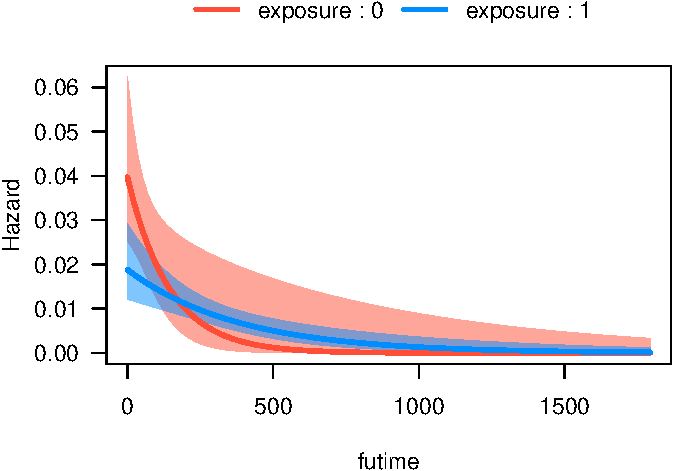
\includegraphics{../figures/stanford-hazard-1} \end{center}

\end{CodeChunk}

The non-proportionality seems to be more pronounced at the beginning of
follow-up than the end. Finally, we can turn these estimate of the
hazard function into estimates of the cumulative incidence functions.

\begin{CodeChunk}

\begin{CodeInput}
R> # Compute absolute risk curves
R> newdata <- data.frame(exposure = c(0, 1))
R> absrisk <- absoluteRisk(fit4, newdata = newdata, 
R+                         time = seq(0, 1000, length.out = 100))
R> 
R> colnames(absrisk) <- c("Time", "NoTrans", "Trans")
R> 
R> # Rearrange the data
R> absrisk <- gather(as.data.frame(absrisk),
R+                   "Status", "Risk", -Time)
R>  
R> ggplot(absrisk, aes(Time, Risk, colour = Status)) +
R+   geom_line() +
R+   theme_minimal() +
R+   theme(legend.position = 'top') +
R+   expand_limits(y = 0.5) +
R+   xlab('Follow-up time') + ylab('Cum. Incidence')
\end{CodeInput}


\begin{center}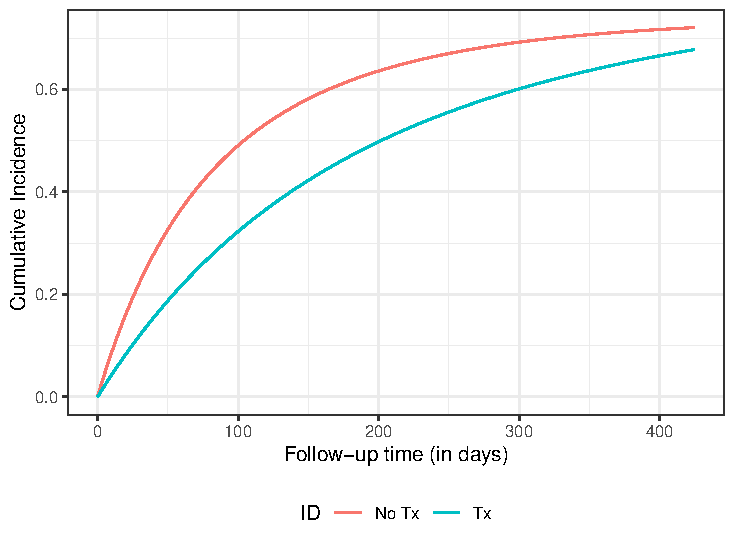
\includegraphics{../figures/stanford-risk-1} \end{center}

\end{CodeChunk}

Note that we can easily adapt the code above to the situation where a
patient receives a heart transplant at a point in time of interest, for
example after 30 days.

\begin{CodeChunk}

\begin{CodeInput}
R> # Compute hazards---
R> # First, create a list of time points for both exposure status
R> one_yr_haz <- data.frame(futime = seq(0, 365,
R+                                       length.out = 100))
R> one_yr_haz <- mutate(one_yr_haz,
R+                      offset = 0,
R+                      exposure = if_else(futime < 30, 0, 1))
R> one_yr_haz$hazard = exp(predict(fit4, newdata = one_yr_haz,
R+                                 type = "link"))
R> ggplot(one_yr_haz, aes(futime, hazard)) +
R+   geom_line() +
R+   theme_minimal() +
R+   theme(legend.position = 'top') +
R+   ylab('Hazard') + xlab('Follow-up time') +
R+   geom_vline(xintercept = 30, linetype = 'dashed')
\end{CodeInput}


\begin{center}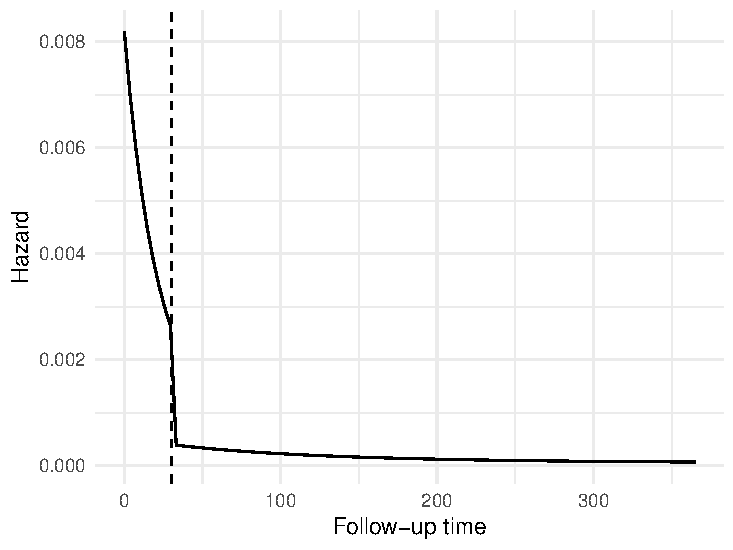
\includegraphics{../figures/stanford-1y-haz-1} \end{center}

\end{CodeChunk}

We can then compare the 1-year mortality risk without transplant and
with transplant at 30 days.

\begin{CodeChunk}

\begin{CodeInput}
R> absoluteRisk(fit4, newdata = data.frame(exposure = 0),
R+              time = 365)
\end{CodeInput}

\begin{CodeOutput}
#>         
#> 365 0.27
\end{CodeOutput}

\begin{CodeInput}
R> 
R> # Use the trapezoidal rule to estimate the cumulative hazard
R> min_hazard <- min(one_yr_haz$hazard)
R> max_hazard <- max(one_yr_haz$hazard)
R> increment <- 365/99
R> cumhaz_est <- 0.5*increment*(sum(2*one_yr_haz$hazard) - min_hazard - max_hazard)
R> 1 - exp(-cumhaz_est)
\end{CodeInput}

\begin{CodeOutput}
#> [1] 0.18
\end{CodeOutput}
\end{CodeChunk}

As we can see, the risk estimate at 1-year is about 30\% lower if the
patient receives a heart transplant at 30 days.

\hypertarget{discussion}{%
\section{Discussion}\label{discussion}}

In this article, we presented the \proglang{R} package \pkg{casebase}
that provides functions to fit smooth parametric hazards and estimate
cumulative incidence functions using case-base sampling. We outlined the
theoretical underpinnings of the approach, we provided details about our
implementation, and we illustrated the merits of the approach and the
package through three case studies.

In the following table we provide a comparison between the Cox model and
case-base sampling:

\hypertarget{environment-details}{%
\section{Environment Details}\label{environment-details}}

This report was generated on 2019-12-05 17:15:04 using the following
computational environment and dependencies:

\begin{CodeChunk}

\begin{CodeInput}
R> # which R packages and versions?
R> devtools::session_info()
\end{CodeInput}

\begin{CodeOutput}
#> - Session info ---------------------------------------------------------------
#>  setting  value                       
#>  version  R version 3.6.1 (2019-07-05)
#>  os       Ubuntu 18.04.3 LTS          
#>  system   x86_64, linux-gnu           
#>  ui       X11                         
#>  language en_CA:en                    
#>  collate  en_CA.UTF-8                 
#>  ctype    en_CA.UTF-8                 
#>  tz       America/Winnipeg            
#>  date     2019-12-05                  
#> 
#> - Packages -------------------------------------------------------------------
#>  package     * version    date       lib
#>  assertthat    0.2.1      2019-03-21 [1]
#>  backports     1.1.5      2019-10-02 [1]
#>  broom         0.5.2      2019-04-07 [1]
#>  callr         3.3.2      2019-09-22 [1]
#>  casebase    * 0.2.1.9001 2019-08-13 [1]
#>  cellranger    1.1.0      2016-07-27 [1]
#>  cli           1.1.0      2019-03-19 [1]
#>  colorspace    1.4-1      2019-03-18 [1]
#>  crayon        1.3.4      2017-09-16 [1]
#>  data.table    1.12.6     2019-10-18 [1]
#>  DBI           1.0.0      2018-05-02 [1]
#>  dbplyr        1.4.2      2019-06-17 [1]
#>  desc          1.2.0      2018-05-01 [1]
#>  devtools      2.2.1      2019-09-24 [1]
#>  digest        0.6.23     2019-11-23 [1]
#>  dplyr       * 0.8.3      2019-07-04 [1]
#>  ellipsis      0.3.0      2019-09-20 [1]
#>  evaluate      0.14       2019-05-28 [1]
#>  farver        2.0.1      2019-11-13 [1]
#>  forcats     * 0.4.0      2019-02-17 [1]
#>  fs            1.3.1      2019-05-06 [1]
#>  generics      0.0.2      2018-11-29 [1]
#>  ggplot2     * 3.2.1      2019-08-10 [1]
#>  glue          1.3.1      2019-03-12 [1]
#>  gtable        0.3.0      2019-03-25 [1]
#>  haven         2.2.0      2019-11-08 [1]
#>  hms           0.5.2      2019-10-30 [1]
#>  htmltools     0.4.0      2019-10-04 [1]
#>  httr          1.4.1      2019-08-05 [1]
#>  jsonlite      1.6        2018-12-07 [1]
#>  knitr         1.26       2019-11-12 [1]
#>  labeling      0.3        2014-08-23 [1]
#>  lattice       0.20-38    2018-11-04 [4]
#>  lazyeval      0.2.2      2019-03-15 [1]
#>  lifecycle     0.1.0      2019-08-01 [1]
#>  lubridate   * 1.7.4      2018-04-11 [1]
#>  magrittr    * 1.5        2014-11-22 [1]
#>  Matrix        1.2-17     2019-03-22 [4]
#>  memoise       1.1.0      2017-04-21 [1]
#>  mgcv          1.8-31     2019-11-09 [4]
#>  modelr        0.1.5      2019-08-08 [1]
#>  munsell       0.5.0      2018-06-12 [1]
#>  nlme          3.1-142    2019-11-07 [4]
#>  pillar        1.4.2      2019-06-29 [1]
#>  pkgbuild      1.0.6      2019-10-09 [1]
#>  pkgconfig     2.0.3      2019-09-22 [1]
#>  pkgload       1.0.2      2018-10-29 [1]
#>  prettyunits   1.0.2      2015-07-13 [1]
#>  processx      3.4.1      2019-07-18 [1]
#>  ps            1.3.0      2018-12-21 [1]
#>  purrr       * 0.3.3      2019-10-18 [1]
#>  R6            2.4.1      2019-11-12 [1]
#>  Rcpp          1.0.3      2019-11-08 [1]
#>  readr       * 1.3.1      2018-12-21 [1]
#>  readxl        1.3.1      2019-03-13 [1]
#>  remotes       2.1.0      2019-06-24 [1]
#>  reprex        0.3.0      2019-05-16 [1]
#>  rlang         0.4.2      2019-11-23 [1]
#>  rmarkdown     1.18       2019-11-27 [1]
#>  rprojroot     1.3-2      2018-01-03 [1]
#>  rstudioapi    0.10       2019-03-19 [1]
#>  rticles       0.12       2019-11-12 [1]
#>  rvest         0.3.5      2019-11-08 [1]
#>  scales        1.1.0      2019-11-18 [1]
#>  sessioninfo   1.1.1      2018-11-05 [1]
#>  stringi       1.4.3      2019-03-12 [1]
#>  stringr     * 1.4.0      2019-02-10 [1]
#>  survival    * 2.44-1.1   2019-04-01 [4]
#>  testthat      2.3.1      2019-12-01 [1]
#>  tibble      * 2.1.3      2019-06-06 [1]
#>  tidyr       * 1.0.0      2019-09-11 [1]
#>  tidyselect    0.2.5      2018-10-11 [1]
#>  tidyverse   * 1.3.0      2019-11-21 [1]
#>  usethis       1.5.1      2019-07-04 [1]
#>  vctrs         0.2.0      2019-07-05 [1]
#>  VGAM          1.1-2      2019-11-21 [1]
#>  withr         2.1.2      2018-03-15 [1]
#>  xfun          0.11       2019-11-12 [1]
#>  xml2          1.2.2      2019-08-09 [1]
#>  yaml          2.2.0      2018-07-25 [1]
#>  zeallot       0.1.0      2018-01-28 [1]
#>  source                                  
#>  CRAN (R 3.6.1)                          
#>  CRAN (R 3.6.1)                          
#>  CRAN (R 3.6.1)                          
#>  CRAN (R 3.6.1)                          
#>  Github (sahirbhatnagar/casebase@aecb816)
#>  CRAN (R 3.6.1)                          
#>  CRAN (R 3.6.1)                          
#>  CRAN (R 3.6.1)                          
#>  CRAN (R 3.6.1)                          
#>  CRAN (R 3.6.1)                          
#>  CRAN (R 3.6.1)                          
#>  CRAN (R 3.6.1)                          
#>  CRAN (R 3.6.1)                          
#>  CRAN (R 3.6.1)                          
#>  CRAN (R 3.6.1)                          
#>  CRAN (R 3.6.1)                          
#>  CRAN (R 3.6.1)                          
#>  CRAN (R 3.6.1)                          
#>  CRAN (R 3.6.1)                          
#>  CRAN (R 3.6.1)                          
#>  CRAN (R 3.6.1)                          
#>  CRAN (R 3.6.1)                          
#>  CRAN (R 3.6.1)                          
#>  CRAN (R 3.6.1)                          
#>  CRAN (R 3.6.1)                          
#>  CRAN (R 3.6.1)                          
#>  CRAN (R 3.6.1)                          
#>  CRAN (R 3.6.1)                          
#>  CRAN (R 3.6.1)                          
#>  CRAN (R 3.6.1)                          
#>  CRAN (R 3.6.1)                          
#>  CRAN (R 3.6.1)                          
#>  CRAN (R 3.5.1)                          
#>  CRAN (R 3.6.1)                          
#>  CRAN (R 3.6.1)                          
#>  CRAN (R 3.6.1)                          
#>  CRAN (R 3.6.1)                          
#>  CRAN (R 3.6.1)                          
#>  CRAN (R 3.6.1)                          
#>  CRAN (R 3.6.1)                          
#>  CRAN (R 3.6.1)                          
#>  CRAN (R 3.6.1)                          
#>  CRAN (R 3.6.1)                          
#>  CRAN (R 3.6.1)                          
#>  CRAN (R 3.6.1)                          
#>  CRAN (R 3.6.1)                          
#>  CRAN (R 3.6.1)                          
#>  CRAN (R 3.6.1)                          
#>  CRAN (R 3.6.1)                          
#>  CRAN (R 3.6.1)                          
#>  CRAN (R 3.6.1)                          
#>  CRAN (R 3.6.1)                          
#>  CRAN (R 3.6.1)                          
#>  CRAN (R 3.6.1)                          
#>  CRAN (R 3.6.1)                          
#>  CRAN (R 3.6.1)                          
#>  CRAN (R 3.6.1)                          
#>  CRAN (R 3.6.1)                          
#>  CRAN (R 3.6.1)                          
#>  CRAN (R 3.6.1)                          
#>  CRAN (R 3.6.1)                          
#>  CRAN (R 3.6.1)                          
#>  CRAN (R 3.6.1)                          
#>  CRAN (R 3.6.1)                          
#>  CRAN (R 3.6.1)                          
#>  CRAN (R 3.6.1)                          
#>  CRAN (R 3.6.1)                          
#>  CRAN (R 3.6.1)                          
#>  CRAN (R 3.6.1)                          
#>  CRAN (R 3.6.1)                          
#>  CRAN (R 3.6.1)                          
#>  CRAN (R 3.6.1)                          
#>  CRAN (R 3.6.1)                          
#>  CRAN (R 3.6.1)                          
#>  CRAN (R 3.6.1)                          
#>  CRAN (R 3.6.1)                          
#>  CRAN (R 3.6.1)                          
#>  CRAN (R 3.6.1)                          
#>  CRAN (R 3.6.1)                          
#>  CRAN (R 3.6.1)                          
#>  CRAN (R 3.6.1)                          
#> 
#> [1] /home/turgeonm/R/x86_64-pc-linux-gnu-library/3.6
#> [2] /usr/local/lib/R/site-library
#> [3] /usr/lib/R/site-library
#> [4] /usr/lib/R/library
\end{CodeOutput}
\end{CodeChunk}

The current Git commit details are:

\begin{CodeChunk}

\begin{CodeInput}
R> # what commit is this file at? 
R> git2r::repository(here::here())
\end{CodeInput}

\begin{CodeOutput}
#> Local:    review-max /home/turgeonm/Documents/git_repos/cbpaper
#> Head:     [77f5e41] 2019-08-02: fix overlapping author names
\end{CodeOutput}
\end{CodeChunk}

\bibliography{references.bib}


\end{document}

